\chapter{Supervised Recurrent Networks}\label{ch_supervised_recurrent}
\chapterauthor{Jeff Yoshimi}

In chapter \extref{ch_intro} we introduced the distinction between feed-forward and recurrent networks, and used that distinction to organize much of this book. Feed-forward networks have historically been a focus of research activity and applications. They are easy to analyze as function approximators or pattern associators which  associate vectors with vectors, and powerful methods like backprop (and the variants used to train deep networks) have emerged to allow them to approximate arbitrary functions (chapter \extref{ch_supervised_ff}). They also produce interesting representations in their hidden layers. As a  result they have often dominated the conversation.

% TODO: If glossary items for generative and discriminative are added, use them here
But recurrent networks have many advantages. Rather than just statically producing a single output for each input, recurrent networks \emph{process} information, producing dynamically changing patterns of activity over time.\footnote{A way to put the point is in terms of machine learning: feed-forward models tend to be discriminative models, which just  classify inputs and in a sense discriminate them from each other, while recurrent networks are generative models, which can generate long complex sequences. But this is a bit misleading because recurrent networks are also used in discriminative tasks, like recognizing sequences.} Like the brain and mind, they are dynamical systems (chapter \extref{ch_dst}). Every network in the human brain is recurrently connected and will produce patterns of activity when stimulated. They are also psychologically plausible. In  chapter \extref{ch_intro} we saw that IAC networks like the Jets and Sharks network can respond to questions by a process of spreading activation in a recurrent connectionist network. In chapter \extref{ch_unsupervised_recurrent} we saw that recurrent networks can be trained using unsupervised methods (like the Hebb rule) to produce fixed point attractors that correspond to memories. 
% The main ones are kind of recurrent, but also kind of ff.

In recent years there has been an explosion of interest in recurrent neural networks or ``RNNs'', based on the adaptation of supervised learning methods discussed in chapters \extref{ch_supervised} and \extref{ch_supervised_ff} to recurrent networks. This has made it possible to \emph{train} networks not just to produce sequences of outputs and also respond to sequences of inputs. These  trained recurrent networks are especially useful in natural language processing, and are pervasive in modern technology. Any time you ``google something'', or type in a partial sentence on your cell phone, these RNNs (or closely related algorithms) are at work in the background suggesting text completions. They also automatically classify online movies, help convert speech to text, produce automated summaries of documents, translate between languages, and even create synthetic music or (more disturbingly) convincing fake news articles. 

For the first part of this chapter we develop the basic theory of supervised recurrent networks, starting with an important historical class of model: the simple recurrent network or SRN. This model basically uses some tricks which make it possible to apply classical backprop techniques to recurrent networks. We then show how this basic idea can been pushed to amazing limits, producing some astounding results. Then we discuss how these ideas have been used in connectionists contexts, to show (for example) that human grammar could be learned and might not be innate. Finally, we discuss a different approach to recurrent networks, that has been mosty used in computational neuroscience, to analyze the representational capacities of  arbitrary recurrent networks.
	
\section{Simple Recurrent Networks}

An important early class of supervised recurrent networks is the \glossary{simple recurrent network} or SRN, which  was developed by Jeff Elman \cite{elman1990finding}, a member the original PDP research group  (in fact, they are also sometimes called ``Elman networks''). SRNs are important because (1) they show what the basic approach to training recurrent networks is, and (2) because they were used by connectionists to demonstrate how grammars could be learned by a network. 
% Elman's paper containers the longer history of the method. Jordan had a similar idea but the context layer copied the outputs, not hidden units.

The structure of an SRN is shown in Fig. \ref{SRN_Structure}. It is basically a regular 3-layer feed-forward network trained using backpropagation, with some special machinery for processing temporal context.The special feature is the ``last hidden state'' portion of the input layer, which is always set to the hidden layer activation vector of last time step (in the first time step it is usually just set to the  zero vector).\footnote{ As McClelland says,``The beauty of the SRN is its simplicity. In fact, it is really just a three-layer, feed-forward back propagation network. The only proviso is that one of the two parts of the input to the network is the pattern of activation over the network's own hidden units at the previous time step'' \url{ https://web.stanford.edu/group/pdplab/pdphandbook/handbookch8.html}.} It is a ``copy-back'' of the hidden  layer. Otherwise it is like another part of the input layer, fully connected to the hidden layer. Thus at any time the full input to the network is the current input, {\emph plus some temporal context}. It's a bit like  someone saying "Good times!''. At the moment you hear them say ``times!'' you have some memory of them having just said ``Good''. You  hear ``times!'' in the context of ``Good''. This allows you to distinguish ``good times'' from ``bad times'' from ``crazy times'', etc.\footnote{This idea occurs in philosophy in the work of Edmund Husserl and others who claimed that human experience essentially involves ``time consciousness'', which in turn includes an awareness of what has just-passed and what is about to come (and note that SRNs are usually trained to predict one step in the future). See \url{https://plato.stanford.edu/entries/consciousness-temporal/}.}$^,$\footnote{But note it's not the past input that is remembered, it's the past  hidden state. That hidden state is influenced by the past  input, \emph{and} earlier hidden states. Thus there is a recursive relationship here that allows the temporal influence to extend arbitrarily far back in the past, though the influence is strongest in the recent past.}

\begin{figure}[h]
\centering
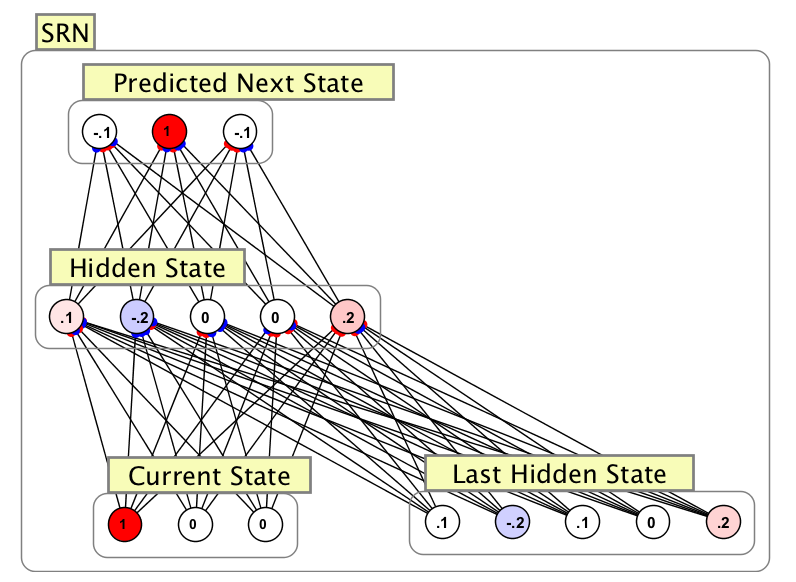
\includegraphics[scale=.6]{./images/srn.png}
\caption[Simbrain screenshot.]{A simple recurrent network.}
\label{SRN_Structure}
\end{figure}

SRNs are also trained in a special way. They use a training dataset, like the ones discussed in chapter \extref{ch_supervised}, and shown below. But unlike a normal training dataset, the rows of an SRN's dataset must be presented in a specific temporal order. As each input vector is presented to the network, the output is computed based on that input vector, \emph{and} on the hidden layer vector from the last time step. Then backprop is used in the usual way to update all the weights of  the network. Here is an example of a training set for a recurrent network. To emphasize the importance of temporal order, a column for time has been added.
 
\begin{center}
\begin{tabular}{| c || c | c | c || c | c | c | }
\cline{1-7}
\multicolumn{1}{| c || }{time} 
& \multicolumn{3}{| c || }{inputs} 
 & \multicolumn{3}{c |}{targets} \\
\hline
1 &  1 & 0 & 0 & 0 & 1 & 0   \\
\hline
2 & 0 & 1 & 0 & 0 & 0 & 1 \\
\hline
3 & 0 & 0 & 1 & 0 & 1 & 0  \\
 \hline
 4 & 0& 1 & 0 & 1 & 0 & 0   \\
\hline
 5 & 1 & 0 & 0 & 0 & 1 & 0  \\
\hline
\end{tabular}
\end{center}

 The dataset above trains an SRN on a one-step prediction problem (which is often what SRNs are used for). It learns to predict the next item in a sequence based on what items have occurred before. In this case it is being trained on a ``bouncing one'' pattern. For example, if we enter $(1,0,0)$, the SRN should predict that $(0,1,0)$  comes next. But notice that the vector $(0,1,0)$ is ambiguous. It will predict \emph{different} outputs depending on when we present it. It predicts  $(1,0,0)$ after  $(0,0,1)$, but  $(0,0,1)$ after  $(1,0,0)$. How can the network do this? Using the context  layer  of course. The last hidden state after seeing $(1,0,0)$ is different then it is after seeing $(0,0,1)$. This allows the network to differentiate the same input, $(0,1,0)$, in different temporal contexts. 
% Alas this is not now working
 
 We can train these networks on arbitrarily long sequences, like all the sentences in a document, or all the images in a movie, or all the sounds in a musical piece, assuming of course that the sentences, images, or sounds have been converted into vectors (see the discussion of feature encoding in chapter \extref{ch_data_science}), though simple SRNs are usually trained on vector encoded text inputs. As we will see, the hidden layer can then be  analyzed for the patterns it discovers and the sequences of patterns it goes through in time.

% Mention simbrain simulations that use this.

\section{Backpropagation  Through Time}

% Discussion of recurrent networks in modern ML often just refer to this.

A more general framework for training recurrent networks (which can be thought of as generalizing the SRN to include arbitrarily many time steps in the past) is by using ``backpropagation through time'' \cite{werbos1990backpropagation}.\footnote{There are other methods of training recurrent networks, eg. real time recurrent learning \cite{williams1989learning}, and ``dynamic reconstruction'' (Haykin, 14.13) \cite{haykin1998neural}.} As with the SRN, we start with a simple three-layer feed-forward network, but instead of a ``copy back''  layer we use a recurrent layer of weights from the hidden layer back to itself. Like the SRN, we have a training dataset that involves time ordered input-target pairs. In order to train the network, we ``unroll'' the network so that all the inputs can be put in the network at the same time. It's as if you take the original network, copy and paste it a bunch of times (once for each row of your training set), and then replace the recurrent weights from the hidden layer back to itself with lateral weights \emph{between} the copy-pasted hidden layers (see figure \ref{bptt}). 

\begin{figure}[h]
\centering
\frame{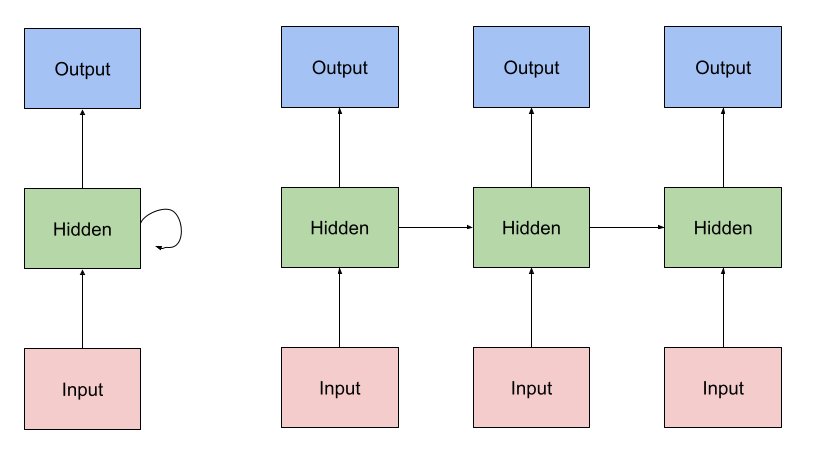
\includegraphics[width=0.5\textwidth]{images/BPTT.png}}
\caption[Jeff Yoshimi.]{Schematic of backprop through time. The actual network that we are training is on the left: a feed-forward network with a recurrent weight layer in the middle. The unrolled network on the right. This network can learn a sequence of three input-target pairs. We train the unrolled network to produced target values in response to current inputs \emph{and} to previous hidden layer states. When training is done, the changes to the weight matrices (the arrows) are added together and so we have ``rolled the network back up'' to the network on the left.}
\label{bptt}
\end{figure}

Each of the unrolled networks is then responsible for a specific moment in time. To train the network we put together all the inputs in the dataset into one long input, one for each of the unrolled networks. Then we train the whole unrolled network in one go, to produce the corresponding sequence of outputs. But you are not just training the usual weights from input-to-hidden layer and from hidden-to-output layer. You are also training the hidden-to-hidden weights in the middle, that laterally connect the hidden layers  of the unrolled network to each other. (Note that the unrolled network is really just a feed-forward network, with some extra lateral weights. So this is ultimately a trick to use feed-forward methods on a recurrent network!) When we are done training this big unrolled network, we add up all the input-to-hidden, hidden-to-hidden, and hidden-to-output weight matrices, which is like collapsing the unrolled network back to down the original network, the one on the left side of figure \ref{bptt}. If we present the network with a sequence of input vectors from the training set, in sequence, it should produce the same sequence of target vectors. And, it should generalize, producing similar sequences of outputs to those in the target set, given a similar sequence of inputs. 

%The network on the left side of figure \ref{bptt} is what the neural network really looks like, the network we will eventually use to do things. Each colored box is a layer of a network, a layer that can have 1 or 2, or maybe 100 or 1000 nodes in it. So this is a kind of zoomed-out view of a 3 layer feed-forward network, where all we see are node layers, not the nodes themselves. The arrows correspond to weight matrices, or weight layers. 

%The unrolled network is on the right. It involves a copy-paste of the same network three times, with the recurrent weights presented as the left-to-right arrows in the middle. Time flows from left to right and each ``column'' (each 2 or 3 layer feed-forward network)  represents one time step. It is being trained on a sequence of three input-target pairs. We present the first input to the first network, compute the output at time 1, then present the second input to the second layer \emph{and also add the activations from the hidden layer at the previous time step}.\footnote{Again, this is a lot like an SRN, since in both cases the hidden layer is receiving a ``visible'' input as well as the hidden layer's previous activation as a second invisible input.}  The output at time 2 then reflects both past inputs: it knows about context. We keep doing this until we reach the end. We have three time steps here, but we can use as many as we have computer memory to handle. Then we train the whole thing with backpropagation. But note, the various arrows on the right side correspond to a bunch of copies of the same weight matrices. So when a pass of training is done, they all get added back together and what we end up with is just the network on the left.

This is a very powerful scheme. Figure \ref{rnn_schema} shows some ways you can use this kind of network. The most general case is shown in the far right panel, where we can imagine that we have a sequence of input vectors, and a sequence of output vectors we'd like to see corresponding to those input vectors. So we train the network to produce that sequence of output vectors in response to that  sequence of input vectors. But of course, we don't have to feed in an input vector at every time step (that is, we can feed in a zero vector sometimes), and  some outputs can be zero vectors that we ignore, so the other panels show some of the other sequencing tasks we can train this kind of network to perform:
\begin{description}
\item[one to many] Example: train a network to produce a bunch of speech from an initial prompt. Give it some initial text and it produces a bunch more.
\item[many to one] Example: train a network to classify a video clip. The video input runs for a while and at the end a classification is output.
\item[many to many] Example: train a network to talk to you while you talk to it.
\end{description}
% Forecasting

\begin{figure}[h]
\centering
\frame{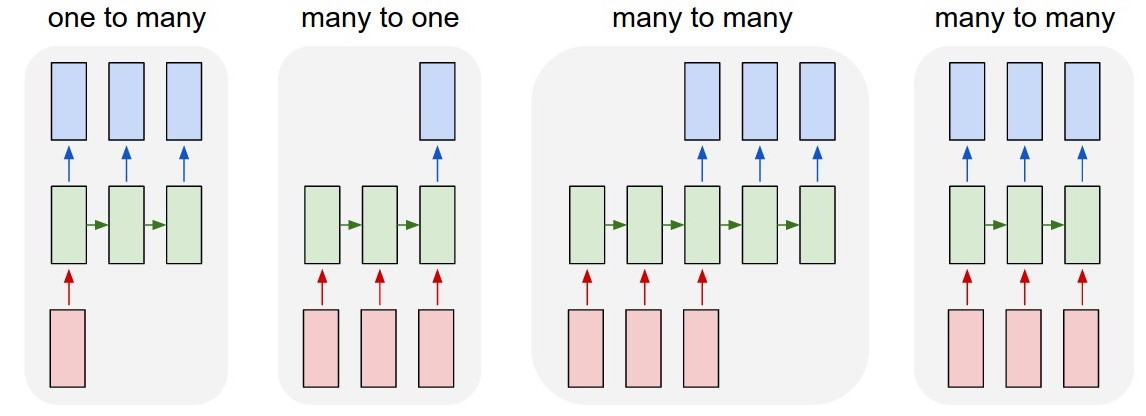
\includegraphics[width=0.7\textwidth]{images/karpathy_rnn.jpeg}}
\caption[From Karpathy, 2015 \cite{karpathy2015unreasonable}.]{Different types of sequence learning possible with backprop through time. }
\label{rnn_schema}
\end{figure}

These ideas have links to dynamical systems theory (chapter \extref{ch_dst}). In the single input or ``one-to-many'' case we are training the network to produce a specific orbit in the output space relative to an initial condition that is produced by the input. Variations on this architecture and this method can be used to train a network to produce a whole phase portrait. In fact, there are theorems which show that recurrent networks can in principle produce any trajectory of any dynamical system \cite{funahashi1993approximation}.\footnote{Even more generally a recurrent network can reproduce any Turing Machine, and hence \emph{any computational system}. They are ``Turing Complete''; see \cite{haykin1998neural} section 15.5; also see  \url{http://binds.cs.umass.edu/papers/1995_Siegelmann_Science.pdf}. These results are comparable to the universal approximation theorem for feed-forward networks noted in chapter \extref{ch_supervised_ff}} 
% Abstractly, that is what is happening with the weird examples in the next section. We train it on some sequences in a linguistic space, etc.

These networks are amazing, as we will see, but they are not perfect. One problem is that they favor recent context over earlier context. But oftentimes it is important to be more sensitive to  information much earlier in a sequence than more recent information, and as a result supervised recurrent networks have a hard time capturing larger temporal structures (like the plot of a story or the overall theme of a musical performance). This is perhaps most clear with certain linguistic tasks, as in the following, due to \cite{mcclelland2020placing}.
\begin{quote}
John put some beer in a cooler and went out with his friends to play volleyball. Soon after he left, someone took the beer out of the cooler. John and his friends were thirsty after the game, and went back to his place for some beers. When John opened the cooler, he discovered that the beer was \rule{1cm}{0.15mm}.
\end{quote}
The reader expects the word ``gone'' next, but if ``took the beer'' is replaced with ``took the ice'' the reader expects something like ``warm''. But the first part of the sentence is too far apart from the last part for an unrolled backprop through time network to pick up the relationship. There are other more technical reasons these networks ran in to trouble, for example the problem of ``vanishing gradients'', which basically means that weights earlier in a temporal sequence get changed much less by the backprop algorithm (and similar algorithms) than weights later in a sequence (further to the left and right of figure \ref{bptt}). 

There have been some successful responses to these issues, like ``long-short-term memories'' or LSTMs (a special kind of circuit that can be trained to hold on to information for long periods)\footnote{See \url{http://colah.github.io/posts/2015-08-Understanding-LSTMs/} \cite{olah2015understanding}}, and more recently transformer architectures which make use of a kind of self-attention \cite{vaswani2017attention}. These architectures have become increasingly prominent and powerful, but they are fairly complex and we will not further develop them here. Discussion of these architectures in relation to cognitive science is in \cite{mcclelland2020placing}.
% Benchmarks that capture this. 
% One shot learning etc.

\section{Text generation with recurrent networks}

% Bring out connection to deep fakes

Supervised recurrent networks can do amazing things, especially when we use powerful computers to train them on a lot of data, for example all the text in Wikipedia, or every math paper in an online database, or all the works of Shakespeare. In a blog post, Andrej Karpathy describes some  simple applications that illustrate the power of supervised recurrent networks.\footnote{\url{http://karpathy.github.io/2015/05/21/rnn-effectiveness/}. Note that Karpathy does train a standard recurrent backprop network, but rather a recurrent network of ``long-short-term memories'' (LSTMs), which have the advantage of being able to track longer term dependencies in a dataset \cite{karpathy2015unreasonable}.}  For example, he trained a neural network on a bunch of Shakespeare\footnote{The data is here: \url{http://cs.stanford.edu/people/karpathy/char-rnn/shakespear.txt}.}  (with words coded as vectors, of course) and then ran  the RNN, which produced it's own version of Shakespeare \cite{karpathy2015unreasonable}. Here is a sample:
% These are called language models. More specifically character level models because they predict the next character in a sequence.

\begin{quotation}
\hspace{5em} \\
VIOLA: \\ \\
\emph{Why, Salisbury must find his flesh and thought \\
That which I am not aps, not a man and in fire, \\
To show the reining of the raven and the wars \\
To grace my hand reproach within, and not a fair are hand}
\end{quotation}
A neural network wrote that! 

\begin{figure}[h]
\centering
\frame{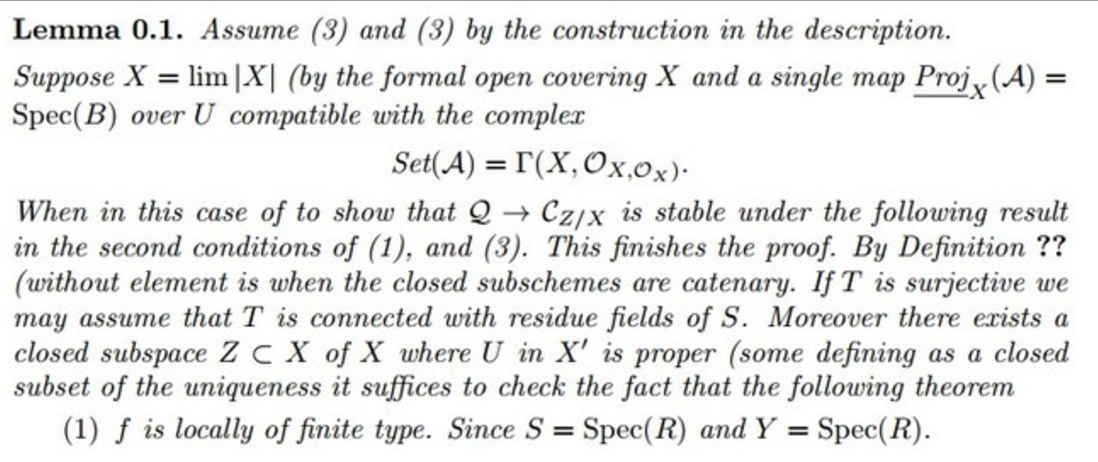
\includegraphics[width=0.7\textwidth]{images/recurrentMath.png}}
\caption[From Karpathy, 2015 \cite{karpathy2015unreasonable}.]{Fragment of ``fake math'' generated by a recurrent network trained on real math.}
\label{fakeMath}
\end{figure}

Karpathy got these supervised recurrent networks to do a bunch of other cool things as well: he generates a fake wikipedia page, a fake math paper, and fake source code \cite{karpathy2015unreasonable}. A fragment from the artificially generated mathematics paper is shown in Fig. \ref{fakeMath}. 

Karpathy also tracked the network's performance during training. Here are a few timeslices of an RNN as it learns to speak like Tolstoy (this network was trained on an English Translation of \emph{War and Peace}):

% https://tex.stackexchange.com/questions/2396/how-can-i-change-the-indentation-in-quote-and-quotation-environments-and-command
\newenvironment{myquote}
  {\list{}{\leftmargin=0.3in\rightmargin=0.3in}\item[]}
  {\endlist}
  
Here it is after iteration 100:
\begin{myquote}
tyntd-iafhatawiaoihrdemot  lytdws  e ,tfti, astai f ogoh eoase rrranbyne 'nhthnee e 
plia tklrgd t o idoe ns,smtt   h ne etie h,hregtrs nigtike,aoaenns ln
\end{myquote}
The network doesn't even really have the concept of a word yet. By iteration 700 it has words, kind of:
\begin{myquote}
Aftair fall unsuch that the hall for Prince Velzonski's that me of
her hearly, and behs to so arwage fiving were to it beloge, pavu say falling misfort 
how, and Gogition is so overelical and ofter.
\end{myquote}
Finally, after a few thousand iterations, it's beginning to sound like a Russian novel:
\begin{myquote}
``Why do what that day,'' replied Natasha, and wishing to himself the fact the
princess, Princess Mary was easier, fed in had oftened him. Pierre asking his soul came to the packs and drove up his father-in-law women.
\end{myquote}

These techniques have even been used to generate a fake script for a movie, which was then actually produced!  The move is called ``Sunspring'', and can be viewed here: \url{https://www.youtube.com/watch?v=LY7x2Ihqjmc}. The opening shows a list of all the other movie scripts that were used to train the network to produce this script \cite{newitz2016movie}.

Karpathy's blog post was written in 2015. In 2020 the power of recurrent networks reached another milestone with the introduction of Open AI's model, GPT-3 \cite{brown2020language, floridi2020gpt}.\footnote{Open AI is a venture launched by Elon Musk and others, and currently funded in part by Microsoft.} This model used all the latest ideas in recurrent neural networks, with a massive dataset, which includes common crawl, which is roughly speaking a web-scraped archive of the \emph{entire internet}. The model has over 175 billion parameters; that is, 175 billion weights and biases! It is absolutely massive, and scary. It arguably passes the Turing Test, a long-standing test for artificial general intelligence, answering questions and producing convincing  text in response to prompts.\footnote{\url{https://plato.stanford.edu/entries/turing-test/}.} For example, when asked to write an article with the title ``United Methodists Agree to Historic Split: Those who oppose gay marriage will form their own denomination'', it produced the following:
\begin{quote}
After two days of intense debate, the United Methodist Church has agreed to a historic split - one that is expected to end in the creation of a new denomination, one that will be ``theologically and socially conservative,'' according to The Washington Post. The majority of delegates attending the church's annual General Conference in May voted to strengthen a ban on the ordination of LGBTQ clergy and to write new rules that will "discipline" clergy who officiate at same-sex weddings. But those who opposed these measures have a new plan: They say they will form a separate denomination by 2020, calling their church the Christian Methodist denomination...
\end{quote}
Most people can't tell that this was written by a computer. Also note that it refers to actual information from online sources,  and that while the other examples from Karpathy feel fake when considered closely, this one does not. GPT-3 is currently being used in hundreds of applications ``around the globe [to]... generate an average of 4.5 billion words per day''.\footnote{From \url{https://openai.com/blog/gpt-3-apps/} retrieved in November 2021. The site also describes some of these applications.} Some philosophical analysis of the promise and potential dangers of this technology are in \cite{floridi2020gpt}.

\section{Connectionist Applications}\label{internalRepsRecurrent}

% Mention psycholinguistis
% ``The paper was ground-breaking for many cognitive scientists and psycholinguists, since it was the first to completely break away from a prior commitment to specific linguistic units (e.g. phonemes or words), and to explore the vision that these units might be emergent consequences of a learning process operating over the latent structure in the speech stream.''

In Chapter \extref{ch_supervised} we saw that multilayer networks trained by supervised learning methods (e.g. backprop) can develop psychologically interesting internal representations that involve a re-mapping of inputs in a hidden layer. Thus backprop is relevant to psychology even if it is not neurally realistic. Similar work has been done with supervised recurrent networks. 

In a famous paper, Jeff Elman trained a simple recurrent network like the one in figure \ref{SRN_Structure} to predict the next words in a sentence.\footnote{\url{http://psych.colorado.edu/~kimlab/Elman1990.pdf}.}  The input data used to train the network consisted of thousands of sentences generated using a simple ``caveman'' grammar. Some sample sentences generated by this grammar are shown in Fig. \ref{elman_sentences}. The network predicts the next word in  a sentence at any time. For example, it predicts that the word ``cat'' will be followed by ``chase'' or ``eat''. With training, error can be reduced, but it never goes to zero, because a given word can be followed by more than one other word. But some words are more likely than others to follow one another, and so the predictions match these patterns. It also learns some general rules, like expecting verbs after nouns \cite{elman1990finding}. 

\begin{figure}[h]
\centering
\frame{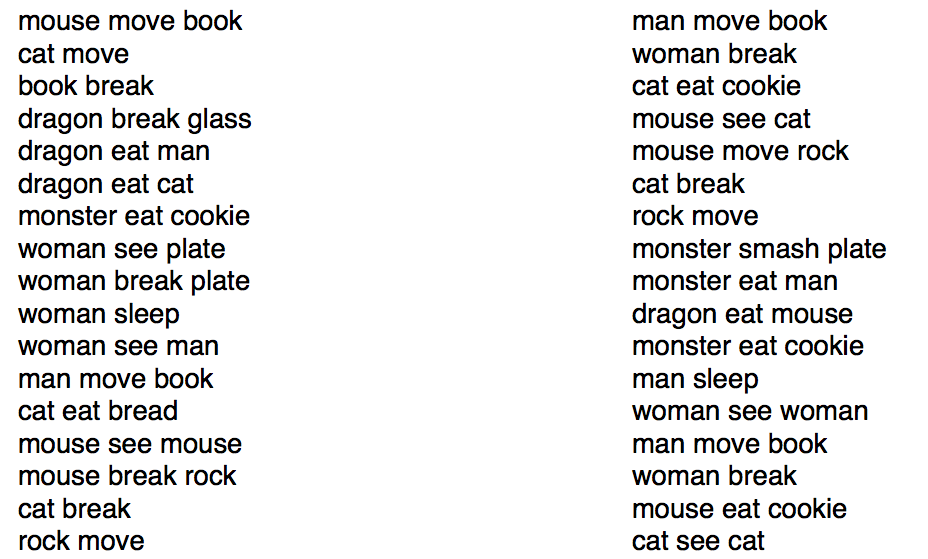
\includegraphics[width=0.65\textwidth]{images/elman_sentences.png}}
\caption[Generated by Jeff Yoshimi based on \cite{elman1990finding}.]{Some of the sentences used to train the word prediction network.}
\label{elman_sentences}
\end{figure}

The striking thing about this network was that it learned a set of grammatical categories in its hidden layer, \emph{without being told anything about grammar}. The internal representations the network learned corresponded to grammatical categories like noun and verb, as well as semantic categories like animal, human, food, and breakable. None of these categories were directly programmed in to the network: it simply learned these categories in the process of solving the input-output task it was given (compare the way Nettalk learned phonological categories when learning to read aloud, or the way deep networks develop realistic edge detectors and other feature detectors when trained to recognize objects). 

Figure \ref{srn_words} shows a schematic reconstruction of the structure of the SRN's hidden unit space.\footnote{The picture this is based on was generated by exposing the network to each word in the context of many sentences (\eg ``eat'', ``cat''), and then taking the average hidden unit activation across these exposures. The resulting vectors are like the centers of clusters in the hidden unit space.} Points correspond to vectors in the hidden unit space. Distances between points are meaningful: points closer to each other in the diagram correspond to hidden unit vectors that are closer to each other in the hidden unit space. Notice that the internal representations form in to a kind of hierarchical structure, that mirrors the structure of English grammar and also some features of English semantics. Nouns are broadly separate from verbs. Within nouns we have animate vs. inanimate nouns. 

This  was a big deal, because it argued against the prevailing view in psycholinguistics, associated with Noam Chomsky,  that  grammars are innate, rather than learned. This provides some evidence for the opposite conclusion. The rules of grammar were not given to the network. They were learned by the network when it was trained to predict the next word in grammatical sentences \cite{elman1990finding}. The grammar was in the sentences, and then learned by the network.
% Written quickly; carefully revise and add citations before publication.

\begin{figure}[h]
\centering
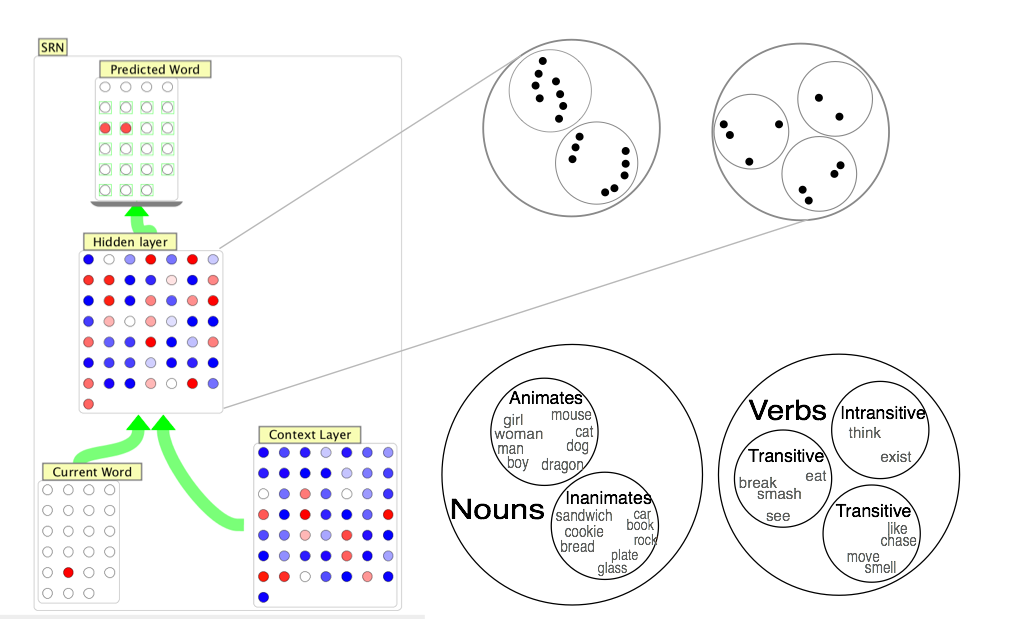
\includegraphics[width=0.7\textwidth]{images/elmanCategories.png}
\caption[Pamela Payne.]{The SRN used in the word prediction task. The output layer predicts the next word (coded as a binary vector) in a sentence. It is currently undecided between which of two words might come next. The right top panel shows (schematically, this is not a projection of actual data) what points in the hidden unit space corresponding to different words. The right bottom panel shows how these points cluster in to grammatical and semantic categories.}
\label{srn_words}
\end{figure}

This is a good example of connectionism. Elman used backprop to show neurally plausible processes could capture psycho-linguistic phenomena, without claiming to show exactly what was happening in the brain.

A final, more recent example, shows that these ideas persist, even among those who are not concerned with cognitive science or psychology. Karpathy's amazing recurrent neural networks, which learned to generate fake math texts, encyclopedia pages, and source code, were also analyzed for internal representations. The results were fascinating. Some nodes only turned on when the network was producing text inside of quotations. Other nodes only turned on at the beginnings and ends of lines. Other nodes kept track of things like opening and closing brackets or parentheses. And yet other nodes produced activity that was hard to interpret. This is a lot like the brain, actually; some nodes seem to code for inputs in a meaningful way (\eg nodes that respond to faces or edges), but others have much more complex response profiles \cite{karpathy2015visualizing}. 